
%% limited to 12 pages, to format use commands:

%% pdflatex main
%% bibtex main
%% pdflatex main
%% pdflatex main

%% view main.pdf with your favorite pdf viewer....

%% OK, for the ACM SIG formatting we have to use latex and dvips to get the
%% desired output.  in particular they suggest the following dvips command be
%% used:

%%ps2pdf14 -dPDFSETTINGS=/prepress pads028-wilsey.ps

\documentclass{sig-alternate}

\usepackage{url}

\begin{document}

%%\conferenceinfo{SIGSIM-PADS'13,} {May 19--22, 2013, Montréal, Québec, Canada.} 
\CopyrightYear{2014} 
%%\crdata{978-1-4503-1920-1/13/05} 
\clubpenalty=10000 
\widowpenalty = 10000

\title{Experiments with Transactional Memory for Event Pool Management}

\numberofauthors{2} 

\author{
\alignauthor
Joshua A. Hay \\
       \affaddr{Dept of of Electrical Engineering and Computing Systems}\\
       \affaddr{Cincinnati, OH  45221-0030}\\
       \email{hayjo813@gmail.com}
\alignauthor
Philip A. Wilsey \\
       \affaddr{Dept of of Electrical Engineering and Computing Systems}\\
       \affaddr{Cincinnati, OH  45221-0030}\\
       \email{wilseypa@gmail.com}
}

\maketitle

\begin{abstract}

%% PHIL: will write this


\end{abstract}

\category{D.1.3}{Programming Techniques}{Concurrent Programming}[parallel
  programming, distributed programming]

\category{I.6.8}{Simulation and Modeling}{Types of Simulation}[parallel,
  distributed, discrete event]

\terms{Algorithms, Performance}

\keywords{Time Warp, pending event lists, multi-core, threads, transactional memory} 

\section{Introduction}\label{introduction}

%% PHIL: will write this


The remainder of this manuscript is organized as follows.  
Section \ref{related} provides a brief review of related studies with
transactional memory.  
Section \ref{background}
provides some background on Time Warp and transactional memory.
Section \ref{warped} reviews the software
architecture of the Time Warp simulation kernel (\textsc{warped}) that is used
in this work and presents some data showing how contention for the shared
pending event set negatively impacts performance.  
Section \ref{experiments} presents the results of our
experimental analysis.  
Finally,Section \ref{conclusions} presents some concluding remarks.

\section{Related Work}\label{related}

%% JOSH: will write this
%% review any studies with transactional memory; especially performance
%% studies.  even studies with software based transactional memory solutions.
%% this should be reasonably short .5 to 1 page

\section{Background}\label{background}

\subsection{The Time Warp Mechanism}

%% PHIL: will write this

\subsection{Transactional Memory}

%% JOSH: will write this
%% describe transactional memory (both the idea and the description of what
%% hardware platforms support transactional memory).  ideally less than one
%% page, but whatever it takes to be complete.


\section{\textsc{warped}: A Time Warp Simulation Kernel}\label{warped}

%% PHIL: will rewrite this; 

%% JOSH: will help if he has any data from warped that shows how the curves of
%% performance with standard warped fall off as contention grows (phil might be
%% able to pull some data from karthik's old m.s. thesis for this if necessary).


\textsc{warped} is a discrete event simulation kernel that implements the Time
Warp synchronization protocol \cite{martin-96}.  It was originally designed and
optimized for executing parallel simulations on a Beowulf Cluster containing
single core processors.  It is highly configurable and incorporates many
different sub-algorithms (\emph{e.g.,} periodic checkpointing
\cite{fujimoto-90}, and lazy, aggressive, and dynamic cancellation
\cite{rajan-95}) of the Time Warp mechanism \cite{fujimoto-90}.  Structurally,
the Logical Processes (LPs) of a simulation are grouped together on each
processing node where the LPs are scheduled according to a Least-Timestamp-First
(LTSF) event scheduling policy.  The node architecture reduces the Time Warp
housekeeping functions such as GVT estimation, termination detection, and fossil
collection into a set of common services for the entire population of LPs on
that node.  This architecture is similar to that reported in \cite{avril-95} and
\cite{ramanan-97}.

\begin{figure*}
  \centerline{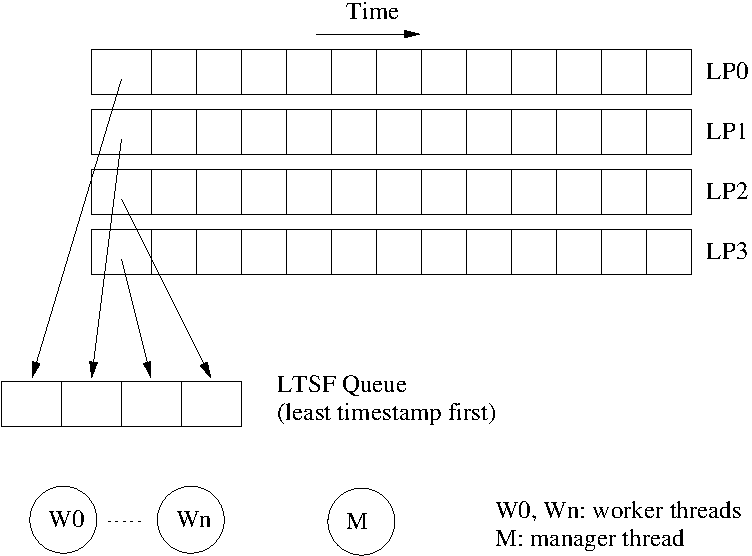
\includegraphics[width=4in]{figs/warpedLTSF}}
  \caption{The principle pending event queues in \textsc{warped}.}\label{warpedLTSF} 
\end{figure*}

Most recently several attempts to build a threaded extension of \textsc{warped}
have been pursued \cite{miller-10,karthik-12}.  These studies have produced a
solution that works reasonably well for smaller multi-core processors.  The
overall design structure depicting the main pending event pool and the executing
threads is shown in Figure \ref{warpedLTSF}.  A threaded instance of
\textsc{warped} contains a manager thread and one or more worker threads.  The
\emph{manager thread} (labeled \texttt{M} in Figure \ref{warpedLTSF}) processes
the Time Warp housekeeping functions and also processes the receipt and
transmission of event messages exchanged with remote nodes in the cluster (local
event insertion is performed by the worker threads).  Additional details on the
operation of the manager thread are available in \cite{karthik-12}.  The
\emph{worker threads} (depicted as \texttt{W0} and \texttt{Wn} in Figure
\ref{warpedLTSF}) are responsible for dequeueing and executing pending events
and generating new events accordingly.  The pending event sets are organized
into a two level structure as described below.

The pending event lists for each LP are maintained as independent
sorted\footnote{Although the prospect of using a partially sorted data structure
  such as calendar queues \cite{brown-88}, lazy queues \cite{ronngren-91}, or
  ladder queues \cite{tang-05} is possible.} lists that are independently
locked.  The lowest timestamped event from each LP event list is placed in a
common LTSF pending event queue.  The (locked) LTSF queue is sorted and used by
the \emph{worker threads} to schedule the next event for execution.  After
dequeuing and processing an event from the LTSF, each worker thread will then
access the pending event set of the LP corresponding to the event just executed
and remove the next least-timestamped event for insertion back into the LTSF
queue.  An abstract representation of the general event processing algorithm
performed by the worker threads is shown in Figure \ref{workerThreadAlgorithm}.

\begin{figure}

\begin{verbatim}
worker_thread()

  lock LTSF queue
  dequeue smallest event from LTSF
  unlock LTSF queue

  while !done loop

    process event (assume from LPi)

    lock LPi queue 

    dequeue smallest event from LPi

    lock LTSF queue

    insert event from LPi
    dequeue smallest event from LTSF

    unlock LTSF queue
    unlock LPi queue
  end loop
\end{verbatim}

\caption{Generalized event execution loop for the worker threads.  Many details
  have been omitted for the sake of clarity.}\label{workerThreadAlgorithm}

\end{figure}

While the above described design works well when the system is configured with
only a few worker threads, once the number of worker threads exceeds 5-6,
contention for the LTSF queue begins to negatively impact performance.  Since
the LP event pools are independently locked and since only one worker thread and
the manager thread will simultaneously access the same LP event pool, contention
to these structures is minimized.  The principle point of contention for pending
events in this architecture are at the LTSF queue.  Thus, this study examines
alternate designs for organizing the pending event list and especially the LTSF
queue.

\section{Transactional Memory in Haswell}\label{haswell}

%% JOSH: will write this
%% explain how to use transactional memory.  give examples.  this section may be
%% 2-3 pages long

\section{Experimental Analysis}\label{experiments}

%% JOSH will write this; this will be the bulk of the manuscript.  


\section{Conclusions}\label{conclusions}

%% JOSH will write this.....most likely short; .5-1 column of prose on one
%% page. 


\section{Acknowledgments}

Support for this work was provided in part by the National Science Foundation
under grant CNS--0915337.  

\bibliographystyle{abbrv}
\bibliography{refs} 

\balancecolumns

\end{document}
